\chapter{Boundaries, Radiation, and Scattering}
\label{ch:boundaries}

\begin{chapterlead}
Chapters~\ref{ch:light-eigenvalue}--\ref{ch:periodicity} established the
spectral theory of closed or periodic photonic systems, where the
operator $\Mop$ is self-adjoint and the eigenfrequencies are real.
Real photonic structures, however, are rarely closed. Light escapes:
a microcavity leaks, a nanoparticle radiates, a grating diffracts.
The moment we impose outgoing-wave boundary conditions to describe this
radiation, the mathematical framework changes qualitatively.
Eigenfrequencies become complex, modes cease to be normalizable in the
usual sense, and the scattering matrix---with its poles and
zeros---replaces the eigenvalue spectrum as the central object.
The scattering framework developed below connects the Hermitian
foundations of Part~I to the non-Hermitian physics of Part~II.
\end{chapterlead}


%% ================================================================
\section{From cavities to open systems}
\label{sec:open-systems}

A perfectly closed cavity---surrounded by perfect electric conductors
(PEC)---supports a discrete, real spectrum as shown in
Section~\ref{sec:spectrum-types}. No energy leaves or enters the cavity,
and the modes are orthogonal standing waves.

Now remove one mirror, or replace the PEC walls with a finite dielectric
boundary. Energy can escape. A mode that was perfectly trapped at
frequency $\omega_0$ now decays in time at a rate $\gamma$, and the
effective eigenfrequency becomes complex:
\begin{equation}
 \omtil_n = \omega_n - i\gamma_n, \qquad \gamma_n > 0.
 \label{eq:complex-freq}
\end{equation}
The field oscillates at $\omega_n$ and decays as $e^{-\gamma_n t}$.
The quality factor is $\Qfac_n = \omega_n / (2\gamma_n)$: higher $\Qfac$
means slower leakage.

This has mathematical consequences. The complex frequency
signals a fundamental change in the mathematical structure of the
Maxwell eigenproblem. Outgoing-wave boundary conditions render the
operator non-self-adjoint, and the entire machinery of Hermitian spectral
theory---real eigenvalues, orthogonality, completeness, energy inner
product---must be rebuilt. That reconstruction is the subject of
Chapter~\ref{ch:qnm}; here we set the stage by introducing the
scattering matrix and the role of boundary conditions.

\subsection{Energy balance in open systems}
\label{ssec:energy-balance-open}

For a finite region $\Omega$ surrounding the scatterer, the time-averaged
Poynting balance can be written as
\begin{equation}
 -\dv{U}{t}
 = P_{\mathrm{rad}} + P_{\mathrm{abs}},
 \qquad
 P_{\mathrm{rad}}
 = \oint_{\partial\Omega}\langle\mathbf{S}\rangle\cdot\nn\;\dd S,
 \label{eq:poynting-open}
\end{equation}
where $U=\int_\Omega \langle u\rangle\,\dd^3 r$ is the stored
electromagnetic energy and $P_{\mathrm{abs}}$ is the power absorbed by
the material inside $\Omega$. For a closed cavity with PEC walls,
$P_{\mathrm{rad}}=0$ and energy is conserved (or dissipated only by
material absorption). For an open system, $P_{\mathrm{rad}}>0$ represents
power carried away by outgoing waves. This radiation loss is irreversible
in the reduced cavity description and is the physical origin of the
imaginary part of the eigenfrequency.

The energy decay rate of a mode with complex frequency
$\omtil = \omega - i\gamma$ is $2\gamma$, and the time-averaged stored
energy $U$ and radiated power $P_{\mathrm{rad}}$ are related by
\begin{equation}
 \Qfac = \omega\,\frac{U}{P_{\mathrm{rad}} + P_{\mathrm{abs}}}
 = \frac{\omega}{2\gamma}.
 \label{eq:Q-from-power}
\end{equation}
When material absorption is negligible, $\Qfac$ is determined solely by
the radiation loss, which is controlled by the geometry of the cavity
opening and the refractive-index contrast at the boundary.


%% ================================================================
\section{Outgoing-wave boundary conditions}
\label{sec:outgoing-bc}

\subsection{The Silver--M\"uller radiation condition}
\label{ssec:silver-muller}

In an open system, we require that far from the scatterer the
electromagnetic field consist only of outgoing waves. In three
dimensions, this is the \emph{Silver--M\"uller radiation condition}:
\begin{equation}
 \lim_{r\to\infty}\left[
 r\left(\sqrt{\muvac}\,\HH\times\hat{\rr}
 - \sqrt{\epsvac}\,\EE\right)
 \right] = 0,
 \label{eq:silver-muller}
\end{equation}
uniformly in angle. The factor is $r$ in three dimensions because
outgoing spherical waves decay as $1/r$; in two-dimensional cylindrical
problems the corresponding condition uses the $\sqrt{r}$ asymptotic
factor. In one dimension, it reduces to requiring a purely outgoing
traveling wave $e^{+ikr}$ (with our $e^{-i\omega t}$ convention) at large
distances.

The Silver--M\"uller condition is the electromagnetic analogue of the
Sommerfeld radiation condition for scalar waves. It ensures that the
scattered field represents power flowing away from the scatterer,
not toward it---a physical requirement for any passive, causal system.

\subsection{Why outgoing-wave conditions break self-adjointness}
\label{ssec:outgoing-breaks-sa}

Unlike the PEC condition $\nn\times\EE = 0$, the outgoing-wave condition
does not make the surface term in the self-adjointness
proof~\eqref{eq:surface-vanish} vanish. Instead, the outgoing wave carries a
nonzero Poynting flux through any enclosing surface:
\begin{equation}
 \oint_{\partial\Omega}\langle\mathbf{S}\rangle\cdot\nn\;\dd S
 = P_{\mathrm{rad}} > 0.
 \label{eq:radiated-power}
\end{equation}
This radiation loss is the physical mechanism by which openness destroys
self-adjointness. Formally, if we try to verify
$\langle\mathbf{F},\Mop\mathbf{G}\rangle
= \langle\Mop\mathbf{F},\mathbf{G}\rangle$ for two outgoing-wave
solutions, the surface integral~\eqref{eq:surface-vanish} leaves a nonzero
remainder proportional to the cross-flux between $\mathbf{F}$ and
$\mathbf{G}$.

The failure of self-adjointness is not a technicality---it is the
mathematical expression of a deep physical fact: an open system exchanges
energy with its environment, and the environment's degrees of freedom are
not included in the operator $\Mop$. The full system (scatterer plus
radiation field at infinity) is still governed by the self-adjoint Maxwell
operator on all of space, but the reduced description restricted to
the scatterer alone is non-self-adjoint. This is the first instance of
a theme that will recur throughout the book: non-Hermiticity as the price
of a reduced description.

\begin{remark}
The outgoing-wave boundary condition depends on frequency through the
wave vector $k = \omega/c$. This means the eigenproblem is nonlinear in
$\omega$: we cannot simply write $\Mop\HH = \omega^2\HH$ with a fixed
$\Mop$ independent of $\omega$. Instead, for each candidate complex
$\omtil$, the boundary condition changes. This is why the eigenfrequencies
of open systems are called \emph{resonances} rather than eigenvalues in the
strict sense.
\end{remark}


%% ================================================================
\section{The scattering matrix}
\label{sec:smatrix}

\subsection{Definition and physical meaning}
\label{ssec:smatrix-def}

Consider a scatterer illuminated by an incoming wave. The total field is
$\EE = \EE_{\mathrm{in}} + \EE_{\mathrm{sc}}$, where $\EE_{\mathrm{sc}}$
satisfies the outgoing-wave condition. If the scatterer is linear, the
relation between incoming and outgoing wave amplitudes defines the
\emph{scattering matrix} $\Smat(\omega)$.

For a one-dimensional layered structure with waves incident from the left
and right, the $2\times 2$ scattering matrix relates incoming amplitudes
$(a_L^+, a_R^-)$ to outgoing amplitudes $(a_L^-, a_R^+)$:
\begin{equation}
 \begin{pmatrix} a_L^- \\ a_R^+ \end{pmatrix}
 = \Smat(\omega)
 \begin{pmatrix} a_L^+ \\ a_R^- \end{pmatrix}
 = \begin{pmatrix} r_L & t' \\ t & r_R \end{pmatrix}
 \begin{pmatrix} a_L^+ \\ a_R^- \end{pmatrix},
 \label{eq:smatrix-1d}
\end{equation}
where $r_L$, $r_R$ are the reflection coefficients from the left and right,
and $t$, $t'$ are the transmission coefficients. For a reciprocal medium,
$t = t'$; for a $\PT$-symmetric structure, additional constraints apply
(Chapter~\ref{ch:pt-symmetric}).

For a general three-dimensional scatterer with $N$ incoming and outgoing
channels (propagating modes of the surrounding medium), $\Smat$ is an
$N\times N$ matrix. The channels may be angular-momentum partial waves
(for spherical scatterers), waveguide modes (for integrated photonic
circuits), or diffraction orders (for periodic gratings).

The physical content of $\Smat(\omega)$ is a complete input-output
description of the scatterer: given any incident field (decomposed into
channel amplitudes), $\Smat$ determines the scattered field. All
measurable quantities---reflection, transmission, absorption,
scattering cross-sections---can be extracted from $\Smat$.

\begin{figure}[t]
 \centering
 
\includegraphics[width=0.98\textwidth]{fig_f4_scattering_channels.pdf}
 \caption{The scattering matrix as an input--output map. Panel (a) defines the two-channel amplitudes used in Eq.~\eqref{eq:smatrix-1d}. Panel (b) shows the corresponding constraint on scattering eigenvalues: lossless systems place them on the unit circle, passive loss moves them inside, and gain can move them outside. This is the scattering version of the distinction between Hermitian and non-Hermitian Maxwell operators.}
 \label{fig:ch4-scattering-channels}
\end{figure}

\subsection{Unitarity and energy conservation}
\label{ssec:unitarity}

For a lossless scatterer (real $\epsr$ everywhere), conservation of the
time-averaged Poynting flux demands that $\Smat$ be unitary:
\begin{equation}
 \Smat^\adj\,\Smat = \mathbf{I}.
 \label{eq:unitarity}
\end{equation}
This is the scattering-matrix analogue of the self-adjointness of $\Mop$.
Unitarity means that the total outgoing power equals the total incoming
power: no energy is created or destroyed inside the scatterer.

For a scatterer with loss, unitarity is violated in a specific direction:
\begin{equation}
 \Smat^\adj\Smat \le \mathbf{I}
 \qquad (\text{sub-unitary: lossy}),
 \label{eq:sub-unitary}
\end{equation}
meaning the eigenvalues of $\Smat^\adj\Smat$ are all $\le 1$. The
deficit represents absorbed power. For a scatterer with gain,
$\Smat^\adj\Smat$ can have eigenvalues $> 1$: the scatterer amplifies
the incident field. The transition from sub-unitary to super-unitary
$\Smat$ as gain is increased corresponds to the transition from a passive
absorber to an active amplifier, and eventually to a laser when a pole
of $\Smat$ reaches the real frequency axis.

\subsection{Reciprocity in scattering}
\label{ssec:smatrix-reciprocity}

For a reciprocal medium (symmetric $\epsr$ tensor), the scattering matrix
satisfies the symmetry
\begin{equation}
 \Smat^\transpose = \Smat,
 \label{eq:smatrix-reciprocal}
\end{equation}
after appropriate normalization of the channel amplitudes. As discussed in
Section~\ref{sec:reciprocity}, reciprocity is distinct from unitarity
(Hermiticity of the Hamiltonian). A lossy reciprocal scatterer has
$\Smat^\transpose = \Smat$ but $\Smat^\adj\Smat \neq \mathbf{I}$.

The distinction is important because it constrains which non-Hermitian
effects are possible in reciprocal media. For example, reciprocity
guarantees $t_L = t_R$ (equal transmission from both sides), even when the
system has gain and loss that break unitarity and produce
$r_L \neq r_R$ (unequal reflection). The directional reflection asymmetry
exploited by $\PT$-symmetric devices (Chapter~\ref{ch:pt-symmetric}) is
therefore consistent with reciprocity.

\subsection{The optical theorem}
\label{ssec:optical-theorem}

For a single incoming channel, the total scattering cross-section
$\sigma_{\mathrm{sc}}$ and the extinction cross-section
$\sigma_{\mathrm{ext}}$ are related by the optical theorem:
\begin{equation}
 \sigma_{\mathrm{ext}} = \frac{4\pi}{k}\,\Im\!\bigl[f(0)\bigr],
 \label{eq:optical-theorem}
\end{equation}
where $f(0)$ is the forward scattering amplitude and $k = \omega/c$.
Extinction equals the sum of scattering and absorption:
$\sigma_{\mathrm{ext}} = \sigma_{\mathrm{sc}} + \sigma_{\mathrm{abs}}$.
For a passive, lossless scatterer, $\sigma_{\mathrm{abs}} = 0$ and
extinction is purely due to scattering.

The optical theorem is a consequence of unitarity and can be derived
directly from the $\Smat$-matrix formalism. It fails for active
(amplifying) scatterers, where $\sigma_{\mathrm{ext}}$ can become
negative---the scattered field interferes constructively with the incident
field in the forward direction, \emph{increasing} the total power. This
is a scattering-theory signature of gain.


%% ================================================================
\section{Poles, zeros, and resonances}
\label{sec:poles-zeros-ch4}

The scattering matrix $\Smat(\omega)$ is a meromorphic function of the
complex frequency $\omega$. Its singularity structure encodes the
complete physics of the open system.

\subsection{Poles: resonances and quasinormal modes}
\label{ssec:poles}

A \emph{pole} of $\Smat(\omega)$ is a complex frequency $\omtil_n$ at
which the scattering matrix diverges. Physically, this means a nonzero
outgoing field exists with no incoming field---the system radiates
spontaneously. The poles are the resonances (quasinormal-mode
frequencies) of the open system~\cite{vial2014quasimodal}.

For a passive system with no gain, all poles lie in the lower half of
the complex $\omega$ plane ($\Im\omtil < 0$), corresponding to decaying
modes. A pole on the real axis would represent a mode with infinite
lifetime---a bound state or, in special circumstances, a bound state in
the continuum (Chapter~\ref{ch:bic-topology}).

Near a single isolated pole, the scattering matrix has the form
\begin{equation}
 \Smat(\omega) \approx \Smat_{\mathrm{bg}}
 + \frac{\mathbf{A}_n}{\omega - \omtil_n},
 \label{eq:pole-expansion}
\end{equation}
where $\Smat_{\mathrm{bg}}$ is a slowly varying background and
$\mathbf{A}_n$ is the residue matrix, whose rank equals the multiplicity
of the pole. This Breit--Wigner form~\cite{alpeggiani2017quasinormal,sauvan2014modal,lasson2014roundtrip} is the foundation of temporal
coupled-mode theory (Chapter~\ref{ch:maxwell-coupled-modes}).

\subsection{Zeros: coherent perfect absorption}
\label{ssec:zeros}

A \emph{zero} of $\Smat(\omega)$---more precisely, a zero of
$\det\Smat(\omega)$---is a frequency at which a specific combination of
incoming waves produces zero outgoing field. All incident energy is
absorbed. This is \emph{coherent perfect absorption} (CPA)~\cite{sweeney2019perfectly,wang2021coherent}, the
time-reverse of lasing. The interplay of poles and zeros under
$\PT$ symmetry is the subject of Chapter~\ref{ch:poles-zeros}.

For a two-channel system, a zero of $\det\Smat$ requires both the
absorption condition ($\Im\varepsilon > 0$) and the correct phase
relationship between the two input beams. The CPA condition is thus
doubly constrained---in both frequency and input-phase space---making it
more experimentally demanding than simple absorption.

\subsection{Pole--zero structure and causality}
\label{ssec:pole-zero-causality}

Causality constrains the analytic structure of $\Smat(\omega)$: in the
upper half of the complex $\omega$ plane ($\Im\omega > 0$), $\Smat$ must
be analytic and bounded for a passive system. Poles can only appear in
the lower half-plane. If gain is introduced, poles can migrate upward;
when a pole crosses the real axis, the system reaches the lasing
threshold.

The zeros of $\det\Smat$ for a passive system lie in the upper
half-plane (by the time-reversal argument: if the poles of
$\Smat$ are in the lower half-plane, the poles of
$\Smat^{-1}$---which are the zeros of $\det\Smat$---are in the
upper half-plane for a time-reversal-symmetric system). This
pole-zero separation is the scattering-theory version of passivity~\cite{zhao2019connection}.
Chapter~\ref{ch:poles-zeros} shows how gain brings poles and zeros
together, culminating in the CPA-laser point where a pole and a zero
meet on the real axis.


%% ================================================================
\section{The Fabry--P\'erot resonator}
\label{sec:fabry-perot}

The simplest and most instructive open resonator is a one-dimensional
Fabry--P\'erot cavity: two partial mirrors separated by a distance $L$
filled with a medium of refractive index $n$. Despite its simplicity, the
Fabry--P\'erot cavity contains, in miniature, all the essential features of
open-system scattering: complex eigenfrequencies, a meromorphic $\Smat$,
and a connection between poles and transmission resonances.

\subsection{Transfer matrix and scattering matrix}
\label{ssec:fp-transfer}

Each mirror is characterized by reflection and transmission coefficients
$r_j$, $t_j$ ($j = 1,2$). The \emph{transfer matrix} $\Tmat$ relates
the field amplitudes on the left to those on the right through
\begin{equation}
 \Tmat = \Tmat_{\mathrm{mirror},1}\,\Tmat_{\mathrm{prop}}(L)\,
 \Tmat_{\mathrm{mirror},2},
 \label{eq:transfer-fp}
\end{equation}
where $\Tmat_{\mathrm{prop}}(L) = \bigl(\begin{smallmatrix} e^{in\omega L/c} & 0
\\ 0 & e^{-in\omega L/c}\end{smallmatrix}\bigr)$ accounts for propagation over
distance $L$ and each mirror matrix encodes the partial reflection and
transmission. The scattering matrix is obtained from $\Tmat$ by a
standard change of basis~(Appendix~\ref{app:transfer}).

For symmetric mirrors ($r_1 = r_2 = r$, $t_1 = t_2 = t$), the
transmission coefficient is
\begin{equation}
 t_{\mathrm{FP}}(\omega) = \frac{(1-|r|^2)\,e^{in\omega L/c}}
 {1 - r^2\,e^{2in\omega L/c}},
 \label{eq:fp-transmission-coeff}
\end{equation}
and the power transmission is the Airy function:
\begin{equation}
 T(\omega) = |t_{\mathrm{FP}}|^2
 = \frac{(1-|r|^2)^2}
 {1 - 2|r|^2\cos(2n\omega L/c) + |r|^4}
 = \frac{1}{1 + F\sin^2(n\omega L/c)},
 \label{eq:airy}
\end{equation}
where the \emph{coefficient of finesse} is
\begin{equation}
 F = \frac{4|r|^2}{(1-|r|^2)^2}.
 \label{eq:finesse-coeff}
\end{equation}
The finesse $\mathcal{F} = \pi\sqrt{F}/2 = \pi|r|/(1-|r|^2)$
measures the sharpness of the transmission peaks relative to the free
spectral range $\Delta\omega_{\mathrm{FSR}} = \pi c/(nL)$.

\subsection{Resonance condition and complex eigenfrequencies}
\label{ssec:resonance-condition}

The poles of the scattering matrix correspond to the condition
\begin{equation}
 r^2\,e^{2in\omtil L/c} = 1,
 \label{eq:fp-resonance}
\end{equation}
which has solutions at complex frequencies
\begin{equation}
 \omtil_m = \frac{m\pi c}{nL}
 - \frac{ic\ln(1/|r|^2)}{2nL},
 \qquad m = 1,2,3,\ldots
 \label{eq:fp-poles-boundaries}
\end{equation}
for real $r$ with $|r| < 1$. The real part gives equally
spaced resonant frequencies (the free spectral range), and the imaginary
part gives the decay rate $\gamma = c\ln(1/|r|)/(nL)$. The quality
factor is
\begin{equation}
 \Qfac_m = \frac{\omega_m}{2\gamma}
 = \frac{m\pi}{2\ln(1/|r|)}.
 \label{eq:fp-Q}
\end{equation}
Higher-order modes ($m \gg 1$) have higher $\Qfac$ because $\omega_m$
grows while $\gamma$ stays fixed. For high reflectivity ($|r| \to 1$),
$\gamma \to 0$ and $\Qfac \to \infty$: the cavity approaches the
closed-cavity limit, and the eigenfrequencies approach the real axis.

\paragraph{Example.}
A silicon slab in air with $n = 3.5$ and $L = 300\;\mathrm{nm}$ has
Fresnel reflectivity $|r| = |n-1|/(n+1) = 0.556$, giving
$\gamma \approx 1.68 \times 10^{14}\;\mathrm{rad/s}$ and
$\Qfac_1 \approx 2.67$. This very low quality factor reflects
the poor confinement of a bare dielectric slab.
Adding distributed Bragg reflectors increases $|r|$ and pushes the poles
closer to the real axis: the quasinormal-mode picture recovers smoothly
the transition from a leaky slab to a high-finesse cavity.
Chapter~\ref{ch:qnm} develops this example further and connects it to
the full QNM pole structure.

\begin{figure}[t]
 \centering
 
\includegraphics[width=0.98\textwidth]{fig_f4_fabry_perot_airy_poles.pdf}
 \caption{The same Fabry--P\'erot resonances seen on the real axis and in the complex plane. Panel (a) shows the Airy transmission peaks as a function of round-trip phase. Panel (b) shows the corresponding scattering poles: the real parts set the peak positions and the imaginary part sets the linewidth.}
 \label{fig:ch4-fabry-perot-airy-poles}
\end{figure}

\subsection{Connection between poles and transmission peaks}
\label{ssec:poles-transmission}

The transmission peaks of the Airy function~\eqref{eq:airy} occur at real
frequencies $\omega_m = m\pi c/(nL)$, which are the real parts of the
poles~\eqref{eq:fp-poles-boundaries}. The full width at half maximum
(FWHM) of each peak is $\delta\omega \approx 2\gamma$, which is twice
the imaginary part of the pole. Thus the poles of $\Smat$ directly
determine the observable transmission spectrum: their real parts give the
peak positions and their imaginary parts give the peak widths.

This connection between complex poles and real-frequency observables is
general: for any open resonator, the scattering spectrum near a resonance
is a Lorentzian (or Fano) line shape whose parameters are set by the
nearest pole of $\Smat$. The full scattering response is the
superposition of contributions from all poles, weighted by their residues
(the Mittag-Leffler expansion of Chapter~\ref{ch:poles-zeros}).

\begin{booknote}[The Fabry--P\'erot as a non-Hermitian paradigm]
The Fabry--P\'erot resonator is the simplest example of how openness
creates non-Hermiticity. The interior of the cavity is lossless (real
$n$), yet the eigenfrequencies are complex because energy leaks through
the partially reflecting mirrors. This is a concrete realization of the
second of the four roads to non-Hermiticity identified in
Section~\ref{ssec:three-conditions}: the boundary conditions, not the
material, break self-adjointness. The pole structure of $\Smat$
provides a complete description of the resonator's spectral response,
replacing the discrete real eigenvalues of a closed cavity with a
constellation of complex poles in the lower half-plane.
\end{booknote}


%% ================================================================
\section{Scattering cross-sections and the Wigner time delay}
\label{sec:cross-sections}

\subsection{Cross-sections from the $\Smat$ matrix}
\label{ssec:cross-from-s}

For a compact scatterer in free space, the total scattering cross-section
$\sigma_{\mathrm{sc}}$ and the absorption cross-section
$\sigma_{\mathrm{abs}}$ can be expressed in terms of the eigenvalues
$s_n(\omega)$ of the $\Smat$ matrix:
\begin{align}
 \sigma_{\mathrm{sc}} &= \frac{\pi}{k^2}\sum_n |1 - s_n|^2,
 \label{eq:sigma-sc}\\
 \sigma_{\mathrm{abs}} &= \frac{\pi}{k^2}\sum_n (1 - |s_n|^2).
 \label{eq:sigma-abs}
\end{align}
For a unitary $\Smat$, $|s_n| = 1$ and $\sigma_{\mathrm{abs}} = 0$: no
absorption occurs, as expected for a lossless scatterer.

The extinction cross-section is
$\sigma_{\mathrm{ext}} = \sigma_{\mathrm{sc}} + \sigma_{\mathrm{abs}}$,
and the optical theorem~\eqref{eq:optical-theorem} relates it to the
forward scattering amplitude. Near a resonance at $\omtil_n$, the
extinction cross-section exhibits a Lorentzian peak:
\begin{equation}
 \sigma_{\mathrm{ext}}(\omega) \approx \sigma_0
 \frac{\gamma_n^2}{(\omega - \omega_n)^2 + \gamma_n^2},
 \label{eq:resonant-extinction}
\end{equation}
where $\sigma_0$ is the peak cross-section, which can exceed the
geometric cross-section by a factor of order $\Qfac$.

\subsection{The Wigner time delay}
\label{ssec:wigner-delay}

The $\Smat$ matrix also characterizes the temporal response of the
scatterer through the Wigner--Smith time-delay matrix~\cite{raman2010photonic,unknown2018phys}:
\begin{equation}
 Q_{\mathrm{WS}} = -i\,\Smat^\adj\,\dv{\Smat}{\omega}.
 \label{eq:wigner-smith}
\end{equation}
For a unitary $\Smat$, $Q_{\mathrm{WS}}$ is Hermitian, and its
eigenvalues $\tau_n(\omega)$ are real time delays~\cite{lasson2014roundtrip}---the durations for
which an incoming wave packet is trapped inside the scatterer before
being released. Near a resonance, the dominant eigenvalue of
$Q_{\mathrm{WS}}$ is of order the resonance lifetime. With the convention
$\omtil_n=\omega_n-i\gamma_n$, the stored energy decays at rate
$2\gamma_n$, so the energy lifetime is
$\tau_E=1/(2\gamma_n)=\Qfac_n/\omega_n$. Phase-delay conventions can
differ by factors of order unity, but the scaling is the same:
high-$\Qfac$ resonances trap light for long times.

\begin{figure}[t]
 \centering
 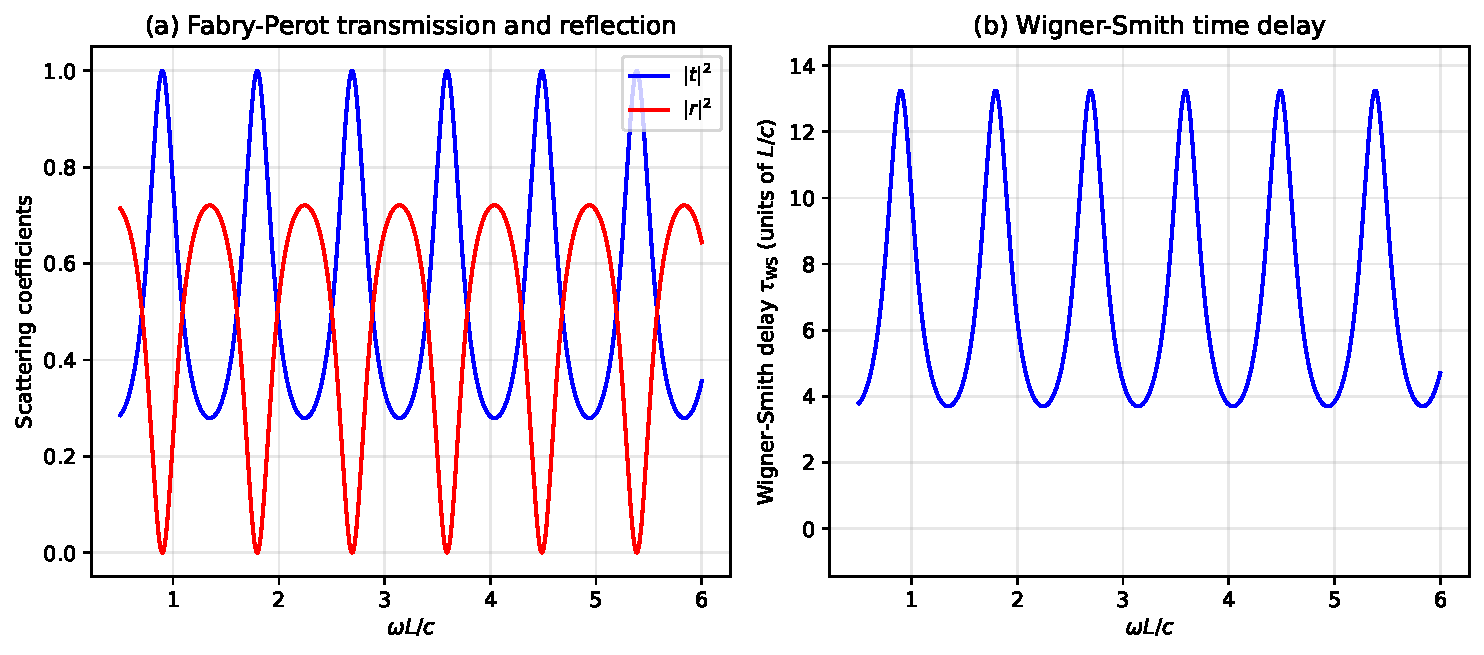
\includegraphics[width=0.85\linewidth]{figures/fig_f04_wigner_smith.pdf}
 \caption{Wigner--Smith time delay for a Fabry--P\'erot cavity
 ($n = 3.5$, $L = 1$).
 (a)~Transmission $|t|^2$ and reflection $|r|^2$ showing the
 characteristic resonance peaks of the etalon.
 (b)~The Wigner--Smith delay
 $\tau_{\mathrm{WS}} = \dd(\arg\det\Smat)/\dd\omega$ peaks sharply
 at each resonance, confirming that high-$\Qfac$ modes trap light for
 long times. Between resonances the delay is small, reflecting the
 short dwell time of off-resonant wave packets.}
 \label{fig:wigner-smith}
\end{figure}

When the $\Smat$ matrix is non-unitary (lossy or amplifying scatterer),
$Q_{\mathrm{WS}}$ is no longer Hermitian, and the time delays become
complex. The imaginary part of the time delay characterizes the
amplification or absorption experienced by the trapped wave packet.
This non-Hermitian time delay is an observable quantity that can be
measured interferometrically and provides a direct experimental
probe of the non-Hermitian character of the scattering process.


%% ================================================================
\section{Spectrum of the open Maxwell operator}
\label{sec:open-spectrum}

For a general open system---not just a Fabry--P\'erot cavity---the
spectrum of the Maxwell operator with outgoing boundary conditions has a
richer structure than the discrete, real spectrum of a closed
cavity~\cite{vial2014quasimodal}.

\paragraph{Discrete resonances.}
The complex eigenfrequencies $\omtil_n$ (poles of $\Smat$) form a
discrete set in the lower half of the complex $\omega$ plane. Near each
pole, the scattered field is dominated by the corresponding quasinormal
mode, whose spatial profile diverges exponentially at infinity (the mode
was excited in the past and its radiation wavefront keeps expanding).

\paragraph{Continuous spectrum.}
In addition to the discrete resonances, the open operator has a
\emph{continuous spectrum} on the real frequency axis, corresponding to
radiation modes that propagate freely in the surrounding medium. These
modes are not square-integrable and cannot be normalized in the same
Hilbert space as bound states.

\paragraph{Bound states and guided modes.}
If the scatterer supports guided modes or bound states (fields that decay
exponentially in all directions without radiation), these appear as
discrete, real eigenfrequencies. They coexist with the continuous
spectrum. In certain symmetry-protected situations, a discrete real
eigenvalue can be embedded \emph{within} the continuous spectrum---a
bound state in the continuum (Chapter~\ref{ch:bic-topology}).

\paragraph{Branch cuts.}
In the complex $\omega$ plane, the continuous spectrum produces branch
cuts rather than isolated singularities. The choice of branch cut
(typically along the negative imaginary axis or the real axis) determines
which Riemann sheet the resonance poles are defined on. This subtlety
becomes important for the mathematical theory of quasinormal-mode
completeness (Chapter~\ref{ch:qnm}).

The full spectral decomposition of the field in an open system requires
all three components: the discrete resonances, the continuous radiation
modes, and any bound states~\cite{vial2014quasimodal}. This is why the
modal theory of open photonic systems is fundamentally different from
that of closed cavities: the resonances alone do not form a complete
basis, and the standard orthogonality relations fail.

\begin{figure}[t]
 \centering
 
\includegraphics[width=0.88\textwidth]{fig_f4_complex_frequency_plane.pdf}
 \caption{Open-system spectra in the complex-frequency plane. Passive
 resonances appear as poles below the real axis; radiation modes form a
 continuum on the real axis; and a guided mode or BIC can remain on the
 real axis without radiating. In a complex-scaled or PML-truncated
 formulation, the radiation continuum is represented by a rotated or
 discretized set of PML modes in the lower half-plane. The marked point
 indicates a continuum threshold or branch point of the radiation channel,
 not an additional resonance of the scatterer. This picture anticipates
 the quasinormal-mode theory of Chapter~\ref{ch:qnm}.}
 \label{fig:ch4-complex-frequency-plane}
\end{figure}


%% ================================================================
\section{Perfectly matched layers}
\label{sec:pml}

\subsection{Complex coordinate stretching}
\label{ssec:pml-stretching}

Numerical computation of resonances requires truncating the infinite
domain to a finite computational region. Simply truncating creates
artificial reflections at the boundary. \emph{Perfectly matched layers}
(PMLs) solve this problem by introducing a complex coordinate
stretching in the outer region that absorbs outgoing waves without
reflection.

In one dimension, the PML replaces the physical coordinate $x$ with
\begin{equation}
 \tilde{x}(x) = x + \frac{i}{\omega}\int_0^x \sigma(x')\;\dd x',
 \label{eq:pml-stretch}
\end{equation}
where $\sigma(x) \ge 0$ is a smooth absorption profile that vanishes
inside the physical domain and grows in the PML region. A plane wave
$e^{ikx}$ in the physical region becomes
$e^{ik\tilde{x}} = e^{ikx}\,\exp\!\bigl(-k\int_0^x\sigma(x')\dd x'/\omega\bigr)$
in the PML region---exponentially decaying for outgoing waves ($k > 0$)
and exponentially growing for incoming waves ($k < 0$). Since only
outgoing waves are present (by the radiation condition), the PML absorbs
all radiation without reflection.

In three dimensions, the PML is implemented by stretching each coordinate
independently:
\begin{equation}
 \tilde{x}_i = x_i + \frac{i}{\omega}\int_0^{x_i} \sigma_i(x_i')\;\dd x_i',
 \qquad i = 1,2,3.
 \label{eq:pml-3d}
\end{equation}
The resulting Maxwell equations in the stretched coordinates have modified
permittivity and permeability tensors that incorporate the PML absorption.

\subsection{Spectral consequences of the PML}
\label{ssec:pml-spectrum}

The PML has a profound consequence for the spectral
theory~\cite{vial2014quasimodal}: the complex coordinate transformation
maps the open Maxwell operator into a \emph{non-self-adjoint operator}
on a bounded domain. The continuous spectrum of the open problem is
rotated into the complex plane by an angle
$\theta_{\mathrm{PML}} = \arctan(\sigma_{\max}/\omega)$, becoming a
discrete set of ``PML modes'' that approximate the radiation continuum.
The true resonances (poles of $\Smat$) are unchanged by the PML---they
are intrinsic to the scatterer---while the PML modes are artifacts of
the truncation, their positions depending on the PML parameters.

This separation is the key to extracting physical information from PML
computations: the physical resonances are identified as eigenvalues that
are insensitive to changes in the PML parameters (thickness, absorption
profile), while the PML modes shift when these parameters are varied.
Chapter~\ref{ch:numerics} discusses practical strategies for
distinguishing physical resonances from PML artifacts.

\subsection{PML as a non-Hermitian mapping}
\label{ssec:pml-nh}

\begin{takeaway}[PML as a non-Hermitian tool]
Perfectly matched layers do more than suppress reflections. They
provide a rigorous non-Hermitian extension of the Maxwell operator that
converts the spectral problem of an open system into a matrix eigenvalue
problem on a bounded domain. The price is non-self-adjointness: the
resulting operator has complex eigenvalues, non-orthogonal eigenvectors,
and requires biorthogonal inner products for modal
expansion~\cite{kristensen2011effective}. This is the starting point
for the quasinormal-mode theory of Chapter~\ref{ch:qnm}.
\end{takeaway}

The PML construction also reveals a deep connection between open
systems and non-Hermitian physics: the radiation boundary condition is
\emph{equivalent} to embedding the scatterer in a non-Hermitian
(absorbing) environment. Whether we model openness as an outgoing-wave
condition at infinity or as a PML-absorbing layer at a finite distance,
the mathematical structure is the same: a non-self-adjoint operator with
complex eigenvalues and biorthogonal modes. The physical content is also
the same: energy leaves the system irreversibly.


%% ================================================================
\section{Feshbach projection and effective non-Hermitian Hamiltonians}
\label{sec:feshbach}

The connection between openness and non-Hermiticity can be made precise
through the Feshbach projection formalism. Partition the full Hilbert
space of the Maxwell operator into a ``system'' subspace $\mathcal{P}$
(e.g., the discrete modes of the cavity) and an ``environment'' subspace
$\mathcal{Q}$ (the continuum of radiation modes):
\begin{equation}
 \hat{P} + \hat{Q} = \mathbf{I}, \qquad
 \hat{P}\hat{Q} = 0.
 \label{eq:feshbach-projection}
\end{equation}
The full eigenvalue problem $\Mop|\psi\rangle = \lambda|\psi\rangle$,
with $\lambda = \omega^2/c^2$, can be projected onto $\mathcal{P}$:
\begin{equation}
 \bigl[\hat{P}\Mop\hat{P}
 + \hat{P}\Mop\hat{Q}\,
 (\lambda - \hat{Q}\Mop\hat{Q})^{-1}\,
 \hat{Q}\Mop\hat{P}\bigr]\,
 \hat{P}|\psi\rangle
 = \lambda\,\hat{P}|\psi\rangle.
 \label{eq:feshbach}
\end{equation}
The term in brackets is an \emph{effective operator} on $\mathcal{P}$
that depends on the eigenvalue $\lambda$. The second term---the
``self-energy'' $\Sigma(\lambda) = \hat{P}\Mop\hat{Q}\,(\lambda -
\hat{Q}\Mop\hat{Q})^{-1}\,\hat{Q}\Mop\hat{P}$---accounts for the
coupling to the radiation continuum. Because the resolvent
$(\lambda - \hat{Q}\Mop\hat{Q})^{-1}$ has poles on the real axis (the
continuous spectrum), $\Sigma(\lambda)$ is complex-valued for real
$\lambda$, and the effective operator is non-Hermitian.

The imaginary part of $\Sigma$ gives the radiative decay rate of the
cavity modes:
\begin{equation}
 \gamma_n = -\Im\!\bigl[\Sigma_{nn}(\omega_n^2/c^2)\bigr],
 \label{eq:feshbach-decay}
\end{equation}
while the real part gives a frequency shift (the Lamb shift analogue in
electrodynamics). The Feshbach formalism thus provides a microscopic
derivation of the complex eigenfrequencies~\eqref{eq:complex-freq}: the
imaginary part arises from the coupling between the cavity modes and the
radiation continuum, not from any material absorption.

This is the fourth road to non-Hermiticity: projection onto a subspace.
Even when the full Maxwell operator is self-adjoint, the effective
operator on a reduced subspace is generically non-Hermitian because the
environment's degrees of freedom carry away energy and information.
Chapter~\ref{ch:maxwell-coupled-modes} develops this idea into the
full temporal coupled-mode theory of photonic resonators.


%% ================================================================
\section{From scattering to non-Hermitian spectral theory}
\label{sec:ch4-forward}

The preceding sections introduced the physical and mathematical framework that
connects closed, Hermitian photonics to the non-Hermitian world:

\begin{itemize}
 \item Outgoing-wave boundary conditions break self-adjointness by
 allowing energy to escape through the surface term in the Poynting
 identity.
 \item The scattering matrix $\Smat(\omega)$, a meromorphic function of
 complex frequency, encodes resonances (poles) and absorption
 conditions (zeros).
 \item Unitarity of $\Smat$ is the scattering analogue of Hermiticity;
 loss or gain breaks unitarity, and the eigenvalues of $\Smat$
 leave the unit circle.
 \item The Fabry--P\'erot resonator illustrates how purely radiative
 loss---without material absorption---creates complex
 eigenfrequencies. The Airy transmission function, the quality
 factor, and the finesse are all determined by the pole structure
 of $\Smat$.
 \item Cross-sections and the Wigner time delay provide measurable
 quantities that are directly expressed in terms of the
 $\Smat$-matrix eigenvalues and their frequency dependence.
 \item Perfectly matched layers provide a rigorous non-Hermitian
 reformulation that enables numerical computation of resonances
 and modal expansions.
 \item The Feshbach projection formalism shows that non-Hermiticity
 arises whenever a self-adjoint system is described by a reduced
 effective operator on a subspace.
\end{itemize}

Chapter~\ref{ch:loss-gain-dispersion} now introduces the complementary
road to non-Hermiticity: material loss, gain, and frequency dispersion.
Chapter~\ref{ch:qnm} develops the full theory of quasinormal modes---the
eigenstates of the non-self-adjoint Maxwell operator with outgoing
boundary conditions---including their normalization, biorthogonality, and
physical applications.
